\documentclass[10pt,twocolumn]{article}
\usepackage[utf8]{inputenc}
\usepackage{amsmath,amssymb}
\usepackage{graphicx}
\usepackage{array}
\usepackage{booktabs}
\usepackage[margin=0.75in]{geometry}
\usepackage{caption}
\usepackage{subcaption}
\usepackage{float}
\usepackage{hyperref}
\usepackage[
    backend=biber,
    style=numeric,
    sorting=none,
    maxbibnames=99,
    giveninits=false
]{biblatex}

% Fix in-text citation format: [Author et al., Year] with hyperlink
\DeclareCiteCommand{\cite}[\mkbibparens]
  {\usebibmacro{prenote}}
  {\usebibmacro{citeindex}%
   \printtext[bibhyperref]{%
     \printnames{labelname}%
     \ifnumgreater{\value{liststop}}{1}{\addspace et al.}{}%
     \addcomma\addspace
     \printfield{year}%
   }}
  {\multicitedelim}
  {\usebibmacro{postnote}}

% Remove the default numeric label completely
\DeclareFieldFormat{labelnumberwidth}{}
\defbibenvironment{bibliography}
  {\list{}
     {\setlength{\leftmargin}{\bibhang}%
      \setlength{\itemindent}{-\leftmargin}%
      \setlength{\itemsep}{\bibitemsep}%
      \setlength{\parsep}{\bibparsep}}}
  {\endlist}
  {\item}

% Create custom bibliography labels: [Author et al., Year]
\renewbibmacro*{begentry}{%
  \mkbibbrackets{%
    \printnames{labelname}%
    \ifnumgreater{\value{liststop}}{1}{\addspace et al.}{}%
    \addcomma\addspace
    \printfield{year}%
  }%
  \addspace
}

% Simplify bibliography entries to match your desired format
\DeclareFieldFormat{title}{#1}  % Remove quotes and italics from title
\DeclareFieldFormat[inproceedings]{title}{#1}
\DeclareFieldFormat{booktitle}{#1}  % Remove italics from booktitle
\DeclareFieldFormat{pages}{pages\addspace#1}  % Add "pages" prefix

% Simplify proceedings entries
\DeclareBibliographyDriver{inproceedings}{%
  \usebibmacro{bibindex}%
  \usebibmacro{begentry}%  % This now prints [Author et al., Year]
  \usebibmacro{author/translator+others}%
  \setunit{\labelnamepunct}\newblock
  \usebibmacro{title}%
  \newunit\newblock
  \usebibmacro{in:}%
  \usebibmacro{maintitle+booktitle}%
  \newunit\newblock
  \printfield{pages}%
  \newunit\newblock
  \usebibmacro{date}%
  \newunit\newblock
  \usebibmacro{finentry}%
}

\addbibresource{refs.bib}

\title{On Smoother Attributions using Neural Stochastic Differential Equations}

\author{
Sumit Jha$^1$, Rickard Ewetz$^2$, Alvaro Velasquez$^3$ and Susmit Jha$^4$ \\
$^1$University of Texas at San Antonio, San Antonio, TX \\
$^2$University of Central Florida, Orlando, FL \\
$^3$Air Force Research Laboratory, Rome, NY \\
$^4$SRI International, Menlo Park, CA \\
sumit.jha@utsa.edu, rickard.ewetz@ucf.edu, alvaro.velasquez.1@us.af.mil, susmit.jha@sri.com
}

\date{}

\begin{document}

\maketitle

\begin{abstract}
Several methods have recently been developed for computing attributions of a neural network's prediction over the input features. However, these existing approaches for computing attributions are noisy and not robust to small perturbations of the input. This paper uses the recently identified connection between dynamical systems and residual neural networks to show that the attributions computed over neural stochastic differential equations (SDEs) are less noisy, visually sharper, and quantitatively more robust. Using dynamical systems theory, we theoretically analyze the robustness of these attributions. We also experimentally demonstrate the efficacy of our approach in providing smoother, visually sharper and quantitatively robust attributions by computing attributions for ImageNet images using ResNet-50, WideResNet-101 models and ResNeXt-101 models.
\end{abstract}

\section{Introduction}
Deep neural networks (DNNs) are increasingly deployed in healthcare, security, autonomous driving, and other safety-critical applications. The responsible use of deep learning in such high-assurance applications necessitates the capability to explain their decisions. However, while a plethora of attribution and explanation techniques have been developed \cite{adebayo2018sanity}, these techniques are known to be noisy and not robust to small input perturbations \cite{adebayo2018sanity}. The noise in pixel-level attributions (Figure 1, center) produced by path-integral-based methods \cite{adebayo2018sanity} has recently been analyzed, and factors such as high manifold curvature and choice of baselines have been identified.

In this paper, we focus on attributions computed over deep learning models that can be analyzed using the theory of dynamical systems \cite{adebayo2018sanity}. Residual neural networks have been modeled using neural ordinary differential equations (ODEs) \cite{adebayo2018sanity}, and stochastic variants of ResNets are described using neural stochastic differential equations (SDEs) \cite{adebayo2018sanity}. We leverage methods from the study of stochastic dynamical systems to show theoretically and empirically that a suitable injection of noise into the residual layers during training produces robust attributions.

\begin{figure}[h!]
\centering
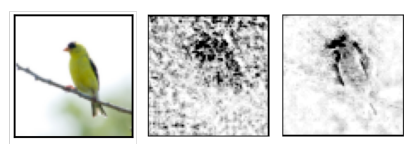
\includegraphics[width=0.48\textwidth]{image.png}
\caption{Input image (left) and results of DeepLIFT SHAP applied to Neural ODEs (center) and Neural SDEs (right). Neural SDEs (right) have visually sharper and less noisy (smoother) attributions.}
\label{fig:main_result}
\end{figure}

We make the following contributions towards computing robust attributions of deep neural network decisions:

1. We perform a worst-case analysis to show that the total attribution computed on neural SDEs trained using noise are more robust than attributions computed on neural ODEs. We are the first to use the connection between dynamical systems and residual neural networks to study the quality of attributions.

2. This robustness of the attributions of our SDE approach is agnostic to the choice of path-integral attribution methods (see tables 1, 2 and 3). We quantitatively demonstrate improvement in the computed attributions using the sensitivity metric [Adebayo et al., 2018].

3. We experimentally illustrate that attributions computed using neural SDEs are qualitatively better, smoother and visually sharper than those obtained from neural ODEs. This improvement is demonstrated on several attribution methods including DeepLIFT SHAP, Smooth-Grad, and Integrated Gradients (see figures 1 through 4).

\section{Overview}
We present a brief summary of our observations and sketch our theoretical analysis as well as our experimental results.

\begin{figure}[h!]
\centering
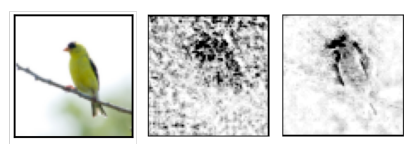
\includegraphics[width=0.48\textwidth]{image.png}
\caption{An overview of our observations and results: ResNets with stochastic noise injected into the residual layers or neural SDEs create more robust attributions. We show that the sum of change in attributions is smaller for neural SDEs than that for neural ODEs.}
\label{fig:overview}
\end{figure}

Given a traditional residual network
\begin{equation}
X(i + 1) = X(i) + R(X(i), W(i)),
\end{equation}
the layers $i$ of the network can be viewed as a time discretization of a continuous neural ODE
\begin{equation}
\frac{dX(t)}{dt} = G(X(t), W(t))
\end{equation}

We suggest the use of neural SDEs
\begin{equation}
dX(t) = G(X(t), W(t)) dt + \sigma(X(t), t) dB(t)
\end{equation}
or ResNets with noise $N(i)$ injected at each residual layer
\begin{equation}
X(i + 1) = X(i) + R(X(i), W(i)) + N(i)
\end{equation}

A natural question to ask is: Can we theoretically and experimentally show that attributions corresponding to neural stochastic differential equations (stochastic ResNets) are inherently more robust that neural ordinary differential equations (ResNets)?

\begin{figure}[h!]
\centering
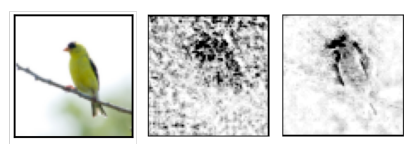
\includegraphics[width=0.48\textwidth]{image.png}
\caption{Input image (left) and results for Integrated Gradients with noise tunnel on neural ODE (center) and the same attribution method applied to our neural SDE (right). The attribution produced by our neural SDE is visibly sharper than the neural ODE attribution.}
\label{fig:ig_comparison}
\end{figure}

\section{Approach and Theoretical Results}

We show that the attributions of neural stochastic differential equations are inherently more robust than the attributions of their deterministic counterparts. In Sec. 3.1, we briefly recapitulate the axiomatic definition of integrated gradients and then review the connection between residual networks with noise and neural stochastic differential equations (SDEs) in Section 3.2 before presenting our theoretical results.

\subsection{Axiomatic Attributions}

In this section, we discuss the axiomatic definition of attributions that will be used in subsequent sections to establish the robustness for neural SDEs. Attribution methods including integrated gradients and Shapley values often employ the notion of a baseline input $x^b$; for example, the all dark image can be a baseline for images. The baseline can also be a set of random inputs where attribution is computed as an expected value.

Let the attribution for the $j$-th feature and output label $i$ be denoted by $A^i_j(x)$. The attribution for the $j$-th input feature depends on the complete input $x$ and not just $x_j$. The treatment for each logit is similar, and so, we can drop the logit/class and denote the network output simply as $F(\cdot)$ and attribution as $A_j(x)$. One can readily make the following two assumptions on the DNN model and the attributions, which reflect that the model is well-trained and the attribution method is well-founded:

1. The attribution is dominated by the linear term. This is also an assumption made by attribution methods based on Shapley values such as Integrated Gradient [Adebayo et al., 2018] which define attribution as the path integral of the gradients of the DNN output with respect to that feature along the path from the baseline $x^b$ to the input $x$, that is,
\begin{equation}
A^i_j(x) = (x_j - x^b_j) \times \int^1_{\alpha=0} \partial_j F^i(x^b + \alpha(x - x^b))d\alpha
\end{equation}
where the gradient of $i$-th logit output of the model along the $j$-th feature is denoted by $\partial_j F^i(\cdot)$.

2. Attributions are complete, that is, the following property is true for any input $x$ and the baseline input $x^b$:
\begin{equation}
F(x) - F(x^b) = \sum^n_{k=1} A_k(x) \text{ where } x \text{ has } n \text{ features.}
\end{equation}

\subsection{Neural Stochastic Differential Equations}

A building block of a residual neural network [Adebayo et al., 2018] with the residual mapping $R(X(i), W(i))$ can be described using the following equation:
\begin{equation}
X(i + 1) = X(i) + R(X(i), W(i))
\end{equation}

The residual network is extended to a stochastic residual network by adding a noise term $N(i)$:
\begin{equation}
X(i + 1) = X(i) + R(X(i), W(i)) + N(i)
\end{equation}

The neural dynamical system corresponding to such stochastic residual networks is obtained by generalizing to a stochastic differential equation [Adebayo et al., 2018]. Here, the noise is modeled by weighing a Brownian motion term $B(t)$ with a suitable diffusion coefficient $\sigma(X(t), t)$:
\begin{equation}
dX(t) = G(X(t), W(t)) dt + \sigma(X(t), t) dB(t)
\end{equation}

\subsection{Robustness of Attributions}

In a neural ODE or SDE, the input $x$ can be denoted by $X(0)$ and the output representation $F(x)$ by $X(t)$. Given a perturbed input $\hat{x}$, the inferred output representation $F(\hat{x})$ of the network may be different from its output representation $F(x)$ to the original input $x$.

\textbf{Theorem 1.} Consider a neural ODE with final output representation $F$ where $\epsilon_x$ denotes a change in the input and $\epsilon_F$ denotes the corresponding change in the output $F$. Similarly, for a neural SDE, we denote the final output representation by $\tilde{F}$, the change in input by $\tilde{\epsilon}_x$, and the change in the final output representation by $\tilde{\epsilon}_F$. The attribution over the inputs for the neural ODE and the neural SDE model is denoted by $A$ and $\tilde{A}$, respectively. The total change in attributions for a neural SDE is smaller than the total change in attributions for a neural ODE for the worst-case input $x$ perturbed to $\hat{x}$, that is,

\begin{equation}
\left\|\sum^n_{k=1} (A_k(\hat{x}) - A_k(x))\right\| \geq \left\|\sum^n_{k=1} (\tilde{A}_k(\hat{x}) - \tilde{A}_k(x))\right\|
\end{equation}

\textbf{Proof.} Given a neural ODE, one can compute a bound on the influence of a small change in the initial input $x$ on the final output representation $F$. $X(t)$ denotes the trajectory starting from the initial state $x$. Let $\hat{C}_F \geq 0$ be a constant bounding the change in the dynamics, that is, for all $t \in [0, T]$, the following holds:
\begin{equation}
\|F(\hat{x}) - F(x)\| \leq \|\hat{x} - x\| e^{\hat{C}_F T} = \epsilon_x e^{\hat{C}_F T}
\end{equation}

From the completeness of attributions for the inputs $x$ and $\hat{x}$, we know the following:
\begin{equation}
F(x)-F(x^b) = \sum^n_{k=1} A_k(x) \text{ and } F(\hat{x})-F(x^b) = \sum^n_{k=1} A_k(\hat{x})
\end{equation}

Subtracting attributions for $x$ from those of $\hat{x}$, we get the following result:
\begin{equation}
\epsilon_F = F(\hat{x}) - F(x) = \sum^n_{k=1} (A_k(\hat{x}) - A_k(x))
\end{equation}

We can similarly bound the change in attributions for the neural SDE. In order to compare a neural ODE and SDE for their relative robustness of attribution, we require them them to be trained with the same data and similar accuracy, except for the insertion of noise in SDEs. Due to this insertion of noise, the dynamics for the training data for neural SDEs will satisfy the following equation
\begin{equation}
\|\tilde{F}(\hat{x}) - \tilde{F}(x)\| \leq \|\hat{x} - x\| e^{(\hat{C}_F + N)T}
\end{equation}
where $N$ depends on the injected noise. Thus,
\begin{equation}
\frac{\epsilon_F}{\epsilon_x} \geq \frac{\tilde{\epsilon}_F}{\tilde{\epsilon}_x}
\end{equation}
because $e^{NT} \geq 1$ since $N$ is positive for any added noise in training the neural SDE.

\section{Experimental Results}

Our attribution analysis and model training is performed on a system with four NVIDIA V100 32GB GPUs using the ResNet-50, WideResNet-101-2 and ResNeXt-101 models [Adebayo et al., 2018] on the ImageNet benchmark. The neural SDE models are trained by injecting a normalized noise into each layer of the residual network. We use the Adam optimizer and the cross-entropy loss in our experimental studies.

\begin{figure}[h!]
\centering
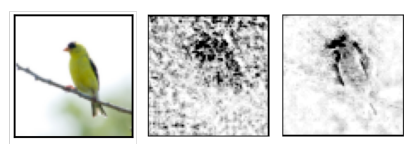
\includegraphics[width=0.48\textwidth]{image.png}
\caption{The top row illustrates the original input image of a digital clock and its attributions using integrated gradients, IG with a noise tunnel, saliency map, DeepLIFT and DeepLIFT SHAP. The visibly best attribution in the top row is obtained by integrated gradient with a noise tunnel and is indicated by a green box. Our neural SDE approach with various normalized magnitudes of noise applied to this attribution method creates a visibly better attribution in the explanation surrounded by a red box.}
\label{fig:digital_clock}
\end{figure}

We use the Captum tool [Adebayo et al., 2018] for computing attributions and use a variety of different attribution methods including integrated gradients, Smoothgrad, DeepLIFT and DeepLIFT Shap to demonstrate the generality of our result. The improvement in attributions for neural SDEs is agnostic to the choice of attribution method.

\subsection{Qualitative Results}

We analyzed attributions for 100 images from the ImageNet validation data set using both Neural ODEs and Neural SDEs for ResNet-50, WideResNet-101-2 and ResNeXt-101 models, and repeated the analysis 5 times to eliminate any significant statistical variations in our quantitative results. Each image has been analyzed using five different attribution methods: integrated gradients [Adebayo et al., 2018], integrated gradients with SmoothGrad [Adebayo et al., 2018], Saliency Maps [Adebayo et al., 2018], DeepLIFT [Adebayo et al., 2018] and DeepLIFT SHAP [Adebayo et al., 2018].

\begin{figure}[h!]
\centering
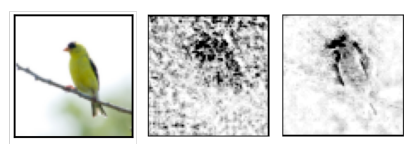
\includegraphics[width=0.48\textwidth]{image.png}
\caption{Neural SDE produces sharper integrated gradients than Neural ODEs. Left to Right: Original image, neural ODE + integrated gradients (IG), neural ODE + IG + noise tunnel, neural SDE + IG + noise tunnel (our approach).}
\label{fig:ig_comparison2}
\end{figure}

\begin{figure}[h!]
\centering
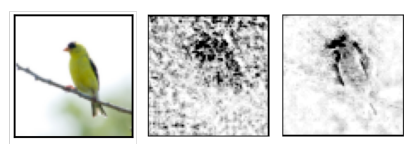
\includegraphics[width=0.48\textwidth]{image.png}
\caption{Neural SDE produces sharper DeepLIFT + SHAP attributions than those produced by Neural ODEs. Left to Right: Original image, neural ODE + DeepLIFT + SHAP, neural SDE + DeepLIFT + SHAP (our approach).}
\label{fig:deeplift_shap}
\end{figure}

\begin{figure}[h!]
\centering
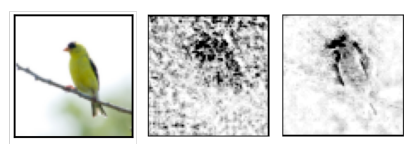
\includegraphics[width=0.48\textwidth]{image.png}
\caption{The DeepLIFT attributions of Neural SDE are visibly sharper than those produced by Neural ODEs. Left to Right: Original image, neural ODE + DeepLIFT, neural SDE + DeepLIFT (our approach).}
\label{fig:deeplift}
\end{figure}

\subsection{Quantitative Results}

We quantitatively study the robustness of the computed attributions for both ResNet-50, WideResNet-101-2 and ResNeXt-101 models using the sensitivity metric [Adebayo et al., 2018] implemented in the Captum library [Adebayo et al., 2018]. We repeated our sensitivity analysis experiments 5 times on 100 correctly labeled but random images from the validation set of the ImageNet benchmark. We report the average values for ResNet-50 in Table 1 below.

\begin{table}[h!]
\centering
\caption{Neural SDE produces a lower sensitivity metric than neural ODE for ImageNet benchmark using the ResNet-50 model.}
\begin{tabular}{p{4cm}lcc}
\toprule
Reference & Attribution & ODE & SDE \\
\midrule
\cite{adebayo2018sanity} & Saliency & 0.5952 & 0.5510 \\
\cite{adebayo2018sanity} & IG & 0.5788 & 0.4498 \\
\cite{adebayo2018sanity} & DeepLIFT & 0.7498 & 0.6134 \\
\cite{adebayo2018sanity} & DeepSHAP & 0.3566 & 0.3230 \\
\bottomrule
\end{tabular}
\label{tab:resnet50}
\end{table}

Table 2 shows the average sensitivity metric obtained from five repetitions of our sensitivity analysis experiments on the WideResNet-101-2 model using both neural ODEs and neural SDEs. The sensitivity metrics [Adebayo et al., 2018] for neural SDEs are smaller than those for neural ODEs.

\begin{table}[h!]
\centering
\caption{The sensitivity metrics for neural SDEs are smaller than those for neural ODEs. Our experiments used the WideResNet-101-2 model and the ImageNet benchmark.}
\begin{tabular}{p{4cm}lcc}
\toprule
Reference & Attribution & ODE & SDE \\
\midrule
\cite{adebayo2018sanity} & Saliency & 0.5972 & 0.5480 \\
\cite{adebayo2018sanity} & IG & 0.5958 & 0.4940 \\
\cite{adebayo2018sanity} & DeepLIFT & 0.8226 & 0.6674 \\
\cite{adebayo2018sanity} & DeepSHAP & 0.3332 & 0.3236 \\
\bottomrule
\end{tabular}
\label{tab:wideresnet}
\end{table}

Table 3 shows the sensitivity metrics obtained from the ResNeXt101 model using both neural ODEs and neural SDEs. Each value for sensitivity metric in the table is an average computed by performing the sensitivity analysis experiments 5 times on 100 ImageNet images.

\begin{table}[h!]
\centering
\caption{Neural SDE produces a lower sensitivity metric than neural ODE for ImageNet using the ResNeXt101 32x8d model.}
\begin{tabular}{p{4cm}lcc}
\toprule
Reference & Attribution & ODE & SDE \\
\midrule
\cite{adebayo2018sanity} & Saliency & 0.6204 & 0.5570 \\
\cite{adebayo2018sanity} & IG & 0.6068 & 0.4976 \\
\cite{adebayo2018sanity} & DeepLIFT & 0.7972 & 0.7130 \\
\cite{adebayo2018sanity} & DeepSHAP & 0.3692 & 0.3302 \\
\bottomrule
\end{tabular}
\label{tab:resnext}
\end{table}

This, our experiments demonstrate that the neural SDEs have lower sensitivity metric than neural ODEs for each of the attribution methods: saliency maps, integrated gradients, Deep LIFT, and DeepLIFT SHAP, and this result generalizes across ResNet-50, WideResNet-101-2 and ResNeXt-101 models.

\section{Related Work}

\textbf{Model interpretability and attribution methods.} A number of techniques [Adebayo et al., 2018] for explaining deep neural networks have recently been proposed in the literature. These methods either provide a complete logical explanation for the output of the model or assign quantitative importance (attributions) to input features for a given model decision.

\textbf{Dynamical systems for neural networks.} Dynamical systems models of neural networks have been the subject of several recent investigations with a particular emphasis on residual networks [Adebayo et al., 2018]. The theory of partial differential equations has been used to obtain dynamical system models of ResNets [Adebayo et al., 2018].

\textbf{Connection between SmoothGrad and our work.} SmoothGrad [Adebayo et al., 2018] uses attributions over multiple noisy variants of an input image to generate visually sharp attributions. Our qualitative experimental results show that neural SDEs lead to SmoothGrad attributions that are visually sharper than SmoothGrad attributions obtained using neural ODEs.

\section{Conclusions}

We make three key observations in this paper. First, we mathematically analyze the attributions computed on neural SDEs trained using noise and show that these are more robust than attributions computed on the deterministic neural ODEs. Second, we experimentally show that this improvement in the computed attributions is agnostic to the choice of path-integral attribution method. We demonstrate improvement over state-of-the-art attribution methods including Saliency Maps, DeepLIFT SHAP and Integrated Gradients (see Fig. 1 through Fig. 4). Finally, we experimentally illustrate that attributions computed using neural SDEs have lower sensitivity scores than those computed using neural ODEs for ResNet-50, WideResNet-101-2 and ResNeXt-101 models.

\section{Acknowledgements}

The authors acknowledge support from the National Science Foundation awards \#2113307, \#1908471, and \#1740079, the DARPA cooperative agreement \#HR00112020002, ONR grant \#N000142112332, and the U.S. Army Research Laboratory Cooperative Research Agreement W911NF-17-2-0196.

\printbibliography

\end{document}